\cleardoublepage
\setcounter{chapter}{1} %The counter for chapters should be set one less than 
                        %the actual chapter number, for example, {1} for 
                        %chapter 2, and {2} for chapter 3.
\setcounter{section}{2} %The counter for sections should be set to match the
                        %actual chapter number, for example, {2} for sections 
                        %in chapter, and {3} for sections in chapter 3. 
\chapter{WebGUI API}
\label{chap:2}
\markboth{WEBGUI USERS' GUIDE}{WEBGUI API}
\pagenumbering{arabic}
\setcounter{page}{3} %The counter for page numbers must be placed here in your
                     %chapter, following the \chapter and \markboth commands.
                     %It should always be the next available right-hand page.
                     %All chapters start on new rights. It will always be
                     %an odd number.  

 
\section{Overview}

\f{WEBGUI} has 19 available functions organized into 4 categories. Each is described in its own section below.\\
\\
\underline{Basic control:}\\
int webstart(int port)\\
void webwriteline(char* str)\\
void webreadline(char* str)\\
void webinit(char* str, int len)\\
void webupdate(int* ip, double* rp, char* sp)\\
void websettitle(char* str)\\
void webstop()\\
\\
\underline{2D Image display:}\\
void websetcolors(int nc, double* R, double* G, double* B, int pane)\\
void webimagedisplay(int nx, int ny, int* image, int pane)\\
\\
\underline{3D Object display:}\\
void websetcolors(int nc, double* R, double* G, double* B, int pane)\\
void webframe(int frame)\\
void weblineflt(float* x, float* y, float* z, int n, int color)\\
void webfillflt(float* x, float* y, float* z, int n, int color)\\
void weblinedbl(double* x, double* y, double* z, int n, int color)\\
void webfilldbl(double* x, double* y, double* z, int n, int color)\\
void webgldisplay(int pane)\\
\\
\underline{Miscellaneous:}\\
int webquery()\\
void webbutton(int highlight, char* cmd)\\
void webpause()\\
void websetmode(int x)\\

\section{Compiling and linking}
The only file that you need to compile and link to your software is webgui.c. No other files are needed. It is true that webgui.c 
mimics a web server and transmits index.html and 3 png images, but these 4 resources are contained within the webgui.c
file as C data.

You can link and subsequently call the external functions of \f{WEBGUI} from any programming language that can
call C language functions. This library has been tested to work with C and Fortran. Compiling, linking, and calling from C
is straight forward. If you wish to compile, link, and call from Fortran, here are some notes.

Every routine described in this section has a matching routine that accepts all the arguments passed as pointers.
For example, the routine \textbf{webstart(int port)} requires that the integer \textbf{port} is passed by value. However
there exists a routine  \textbf{webstart\_(int* port)}  that accepts \textbf{port} as a pointer. All of the twin routines
that accept pointer references have the same function name as the original but end with an underscore.

These matching twin functions are particularly helpful for linking against Fortran. By default, Fortran calls subroutines
by passing pointers for everything. Even if you call \textbf{webstart(15000)} in Fortran, then Fortran will place
the integer 15000 somewhere in memory and pass a pointer to where it resides. That being said, if you wish to link
\f{WEBGUI} to Fortran, you do not need to write an underscore after each routine name. The compiler does this without
you knowing. Here is an example of how you would call \textbf{webstart} with Fortran:
\begin{verbatim}
integer(kind=4) :: port
port = 15000
call webstart(port)
\end{verbatim}
Notice that the call to \textbf{webstart} does not contain a trailing underscore. However the compiler and linker will look
and link this Fortran call to the \f{WEBGUI} routine \textbf{webstart\_} for you.

Fortran differs from C in other ways also. Fortran accesses arrays
starting from index 1 instead of 0. Whenever this is relevent to a routine it is noted in the API. Namely, the routine \textbf{websetcolors}
defines a palette that you later reference from \textbf{webimagedisplay}, \textbf{webline}, and \textbf{webfill}. When referencing
the colors, you refer to the first color as 0 and the second as 1, etc. This is mentioned in the API below. Also, when calling \textbf{webinit}
you declare indices for the parameters. These indices need to match array indices of arguments to \textbf{webupdate}. In this case,
you start indexing from 1. This is explained in the API to follow.

Fortran does not terminate strings (character arrays) with a NULL (char = 0) like C does. Instead Fortran adds space characters
to fill the entire character array after the used portion of the array. All of \f{WEBGUI}'s routines that accept strings will
accept either C or Fortran strings. These routines are \textbf{webwriteline}, \textbf{webinit}, \textbf{webupdate}, \textbf{websettitle},
and \textbf{webbutton}.

If you wish to compile and link against a Fortran program, type something like
\begin{verbatim}
gcc -c webgui.c
gfortran YourProgram.f webgui.o 
\end{verbatim}

When passing arguments, note that the C language variables \textbf{int, float, double, char[80]} are usually 4, 4, 8, 80 bytes 
respectively. When declaring Fortran variables to use as arguments to call \f{WEBGUI} functions, they must be of compatible size. 
To match the former C variables, one typically declares
 \textbf{integer(kind=4), real(kind=4), real(kind=8), character(len=80)} in Fortran respectively. If you wish to capture a return value
 from one of \f{WEBGUI}'s functions, you must make a Fortran function call instead of a Fortran subroutine call and you must declare
 the return value type.
 
 For example, earlier in this section there is an example showing how to call \textbf{webstart} as a Fortran subroutine. To capture
 the return value from \textbf{webstart}, call it as a Fortran function like the following:
 \begin{verbatim}
integer(kind=4) :: webstart
integer(kind=4) :: error 
integer(kind=4) :: port
port = 15000
error = webstart(port)
\end{verbatim}

\newpage
\section{Basic control}
%%%%%%%%%%%%%%%%%%%%%%%%%%%%%%%%%%%%%%%%%%%%%%%%%%%%%%%%%%%%%%%%%%%%%%%%%%%%
% WEBSTART
%%%%%%%%%%%%%%%%%%%%%%%%%%%%%%%%%%%%%%%%%%%%%%%%%%%%%%%%%%%%%%%%%%%%%%%%%%%%
\subsection{webstart}
\underline{Description} The function \textbf{int webstart(int port)} commences the graphical user interface. Specifically
it deploys a web server and creates a new thread which listens for incoming connections on the chosen port.
After calling \textbf{webstart}, any web browser can connect and display the GUI controls by entering your host
computer's URL:port. Afterward, inside the web browser, they will see a pane for displaying text output, three 
panes for displaying graphical output, and either buttons or a space where they can enter string commands. See Figure
\ref{fig:1}. If you wish to have buttons in your GUI, you need to call \textbf{webinit} before this. See Section \ref{sec:2-1}\\
\\
\underline{Declaration} 
\begin{verbatim} 
	int webstart(int port) 
\end{verbatim}
\underline{Parameters} \textbf{port} is a (4 byte) integer which defines which port the web server will listen on.\\
\\
\underline{Return Value} If successful, 0 is returned. On failure, a negative number is returned. -1 indicates that the
requested port is already in use. -2 indicates an inability to create a socket.\\
\\
\underline{Example} The following example shows the usage of \textbf{webstart}.
\begin{verbatim}
#include <webgui.h>
#include <unistd.h>

int main(){
    webstart(15000);
    pause();
    return 0;
}
\end{verbatim}
Assume that your computer's ip address is 172.217.5.206, then after compiling and running the above program.
You can open any web browser and enter the URL = http://172.217.5.206:15000 and your web browser will
display basic controls as displayed in Figure \ref{fig:1}. If your web browser and program are both running
on the same computer, you can use the URL = http://localhost:15000. After calling \textbf{webstart}, the host machine's 
standard output will display:
\begin{verbatim}
webgui: Listening on port 15000 for web browser...
\end{verbatim}
Or you may see the message:
\begin{verbatim}
webgui: FAILURE: server can't bind port 15000
\end{verbatim}
A common \textbf{webstart} error is trying to run two instances of \textbf{WEBGUI} using the same port. 
The second instance will fail. In this case, \textbf{webstart} returns -1. Your 
software should check for this error and act accordingly. Three suggestions are (i) terminate your program,
(ii) wait 5 seconds and try again, or (iii) try binding to a different port. Here is C code that replaces the line 
\textbf{webstart(15000)} in the above example:\\
case i:
\begin{verbatim}
    if (webstart(15000)<0) exit(1);
\end{verbatim}
case ii:
\begin{verbatim}
    while (webstart(15000)<0) sleep(5);
\end{verbatim}
case iii:
\begin{verbatim}
    int offset=0;
    while (webstart(15000+offset)<0) offset++;
\end{verbatim}
In Fortran, you must declare \textbf{webstart} as a 4 byte integer. Here is Fortran code:\\
case i:
\begin{verbatim}
    integer(kind=4) :: webstart
    if (webstart(15000)<0) stop;
\end{verbatim}
case ii:
\begin{verbatim}
    integer(kind=4) :: webstart
    do
        if (webstart(15000)==0) exit;
        call sleep(5)
    end do
\end{verbatim}
case iii:
\begin{verbatim}
    integer(kind=4) :: webstart, offset
    offset=0
    do
        if (webstart(15000+offset)==0) exit;
        offset = offset+1
    end do
\end{verbatim}

\begin{figure}[p!]
\centering
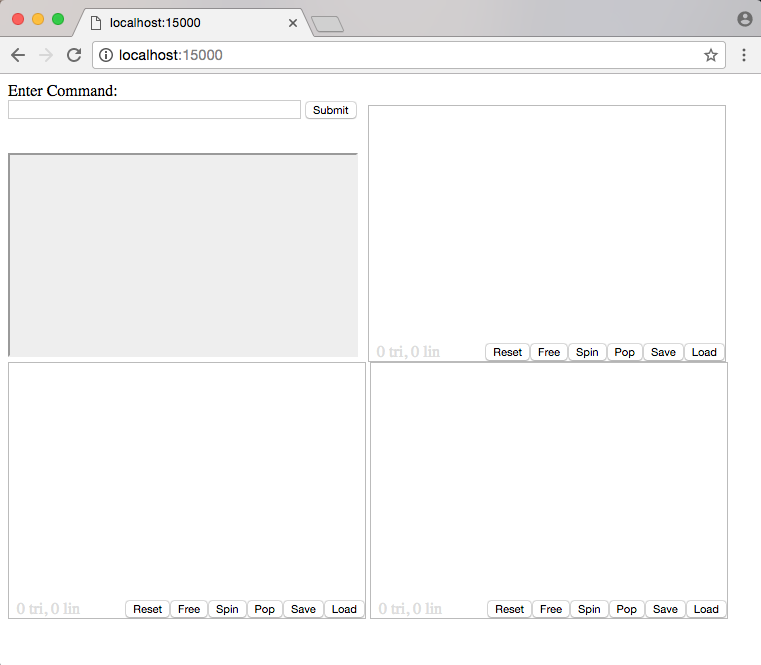
\includegraphics[width=0.75\textwidth]{pix/gui.png}
\caption{\f{WEBGUI} after calling \textbf{webstart}.}
\label{fig:1}
\end{figure} 

%%%%%%%%%%%%%%%%%%%%%%%%%%%%%%%%%%%%%%%%%%%%%%%%%%%%%%%%%%%%%%%%%%%%%%%%%%%%
% WEBWRITELINE
%%%%%%%%%%%%%%%%%%%%%%%%%%%%%%%%%%%%%%%%%%%%%%%%%%%%%%%%%%%%%%%%%%%%%%%%%%%%
\newpage
\subsection{webwriteline}
\label{sec:2-2}
\underline{Description} The function \textbf{void webwriteline(char* str)} displays a line of text in the text
output pane of the web browser graphical interface. \\
\\
\underline{Declaration}
\begin{verbatim} 
	void webwriteline(char* str)
\end{verbatim}
\underline{Parameters} \textbf{str} is a string of length 80. This string can either be null terminated and less than length 80 as is the convention 
of C strings, or the unused characters of the array should be filled with spaces as is the convention of Fortran strings.\\
\\
\underline{Example} The following example shows the usage of \textbf{webwriteline}.
\begin{verbatim}
#include <webgui.h>
#include <unistd.h>

int main(){
    webstart(15000);
    webwriteline("Hello World!");
    pause();
    return 0;
}
\end{verbatim}
After compiling and running the above program, the web browser will show the string, "Hello World!", in
the text output pane (top left pane of 4 panes) as shown in Figure \ref{fig:2}. Below is an alternate example
which accomplishes the same thing.

\begin{figure}[p!]
\centering
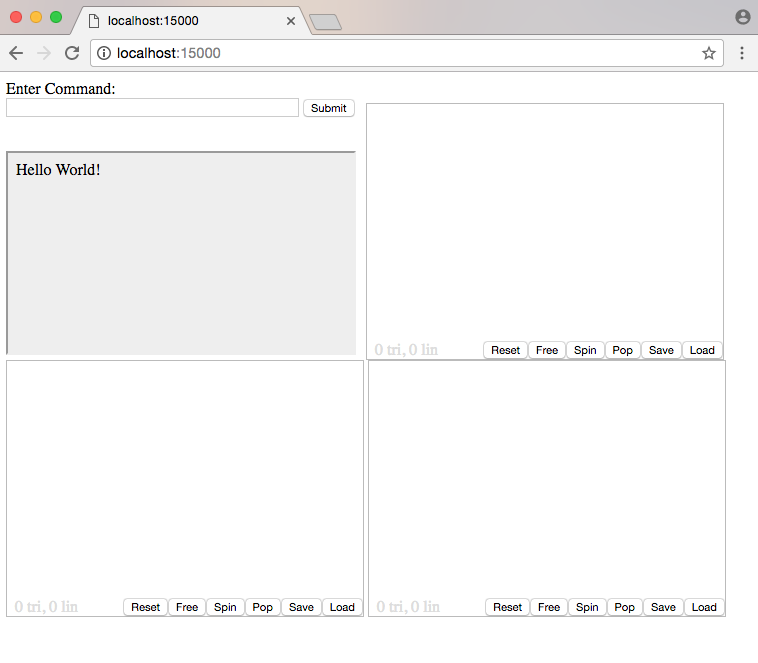
\includegraphics[width=0.75\textwidth]{pix/helloworld.png}
\caption{\f{WEBGUI} after calling \textbf{webwriteline}("Hello World!").}
\label{fig:2}
\end{figure}
\begin{verbatim}
#include <webgui.h>
#include <string.h>
#include <unistd.h>

int main(){
    char str[80];
    strcpy(str,"Hello World!");
    webstart(15000);
    webwriteline(str);
    pause();
    return 0;
}
\end{verbatim}

%%%%%%%%%%%%%%%%%%%%%%%%%%%%%%%%%%%%%%%%%%%%%%%%%%%%%%%%%%%%%%%%%%%%%%%%%%%%
% WEBREADLINE
%%%%%%%%%%%%%%%%%%%%%%%%%%%%%%%%%%%%%%%%%%%%%%%%%%%%%%%%%%%%%%%%%%%%%%%%%%%%
\newpage
\subsection{webreadline}
\label{sec:2-7}
\underline{Description} The function \textbf{void webreadline(char* str)} retrieves the oldest unread string from the
command string queue. If no strings are available, this function call will wait and not return until it receives
a string. Whenever the user submits a command string from the web browser, that string is placed in the command string
queue. If the web browser has buttons showing, pushing the buttons generates a command string as described
in Section \ref{sec:3-3} and places that command string in the queue.\\
\\
\underline{Declaration}
\begin{verbatim} 
	void webreadline(char* str)
\end{verbatim}
\underline{Parameters} \textbf{str} is a char buffer of length 80. After calling \textbf{webreadline}, this buffer
will contain the oldest unread command string. The returned string will not be null terminated as is the convenction
of C strings. Instead the unused portion of the buffer will be filled with the space character as is the convenction of
Fortran strings.\\
\\
\underline{Example} The following example shows the usage of \textbf{webreadline}.
\begin{verbatim}
#include <webgui.h>
#include <stdio.h>

int main(){
    char str[80];
    webstart(15000);
    while(1){
        webreadline(str);
        printf("%.80s\n",str);
    }
    return 0;
}
\end{verbatim}
After compiling and running the above program, the standard output will display any command string(s) that are
submitted by the user in the web browser interface.

%%%%%%%%%%%%%%%%%%%%%%%%%%%%%%%%%%%%%%%%%%%%%%%%%%%%%%%%%%%%%%%%%%%%%%%%%%%%
% WEBINIT
%%%%%%%%%%%%%%%%%%%%%%%%%%%%%%%%%%%%%%%%%%%%%%%%%%%%%%%%%%%%%%%%%%%%%%%%%%%%
\newpage
\subsection{webinit}
\label{sec:2-1}
\underline{Description} The function \textbf{void webinit(char* str, int len)} is called before \textbf{webstart}
if the user wishes to have command buttons on their web browser GUI. Pushing these buttons generates command strings
similar to typing commands when buttons are not present. Additionally, the web browser GUI can store parameter
values associated with your program and allow the user to view and change them. See Section \ref{sec:3-2} for more info.\\
\\
\underline{Declaration}
\begin{verbatim} 
	void webinit(char* str, int len)
\end{verbatim}
\underline{Parameters}\\
\textbf{str} is an array of strings where each string is length 80. These strings can be
either null terminated as is the convention of C strings or they can be padded with spaces as is the convenction
of Fortran strings. However, the second string must start at str[80], and the third string at str[160], etc. A
description on how to format \textbf{str} to create buttons and define parameters can be found in Section \ref{sec:3-2}.\\
\textbf{len} is a (4 byte) integer stating how many strings are present in the array.\\
\\
\underline{Example} The following example shows the usage of \textbf{webinit}.
\begin{verbatim}
#include <webgui.h>
#include <unistd.h>

int main(){
    char str[14][80] = {
        "c c=BuildTire, k=t",
        "c c=BuildEngine, k=e",
        "c c=AssembleCar, k=c",
        "n n=TireRadius, a=tr, t=r, i=1, d=12.5",
        "n n=TireColor, a=tc, t=s, i=1, d=red",
        "n n=EngineSize, a=es, t=i, i=1, d=300",
        "n n=CarColor, a=cc, t=i, i=2, d=1",
        "r c=BuildTire, n=TireRadius",
        "r c=BuildTire, n=TireColor",
        "r c=BuildEngine, n=EngineSize",
        "r c=AssembleCar, n=CarColor",
        "s n=CarColor, v=0, l=red",
        "s n=CarColor, v=1, l=white",
        "s n=CarColor, v=2, l=blue"
    };
    webinit((char*)str,14);
    webstart(15000);
    pause();
    return 0;
}
\end{verbatim}
After compiling and running the above program, the web browser GUI will have 3 command buttons (labeled BuildTire,
BuildEngine, and AssembleCar) and each button will have a drop down menu to view and change associated parameters.
Furthermore, the parameter CarColor (which is in the drop down menu of AssembleCar) will have its own drop down
menu to help select a value. See Figure \ref{fig:3}. Additionally, 4 parameters will be stored in the web browser GUI
(TireRadius, TireColor, EngineSize, and CarColor). These parameters will be viewable and changeable by the user.
To learn more about creating buttons and defining parameters, see Section \ref{sec:3-2}.
\begin{figure}[b!]
\centering
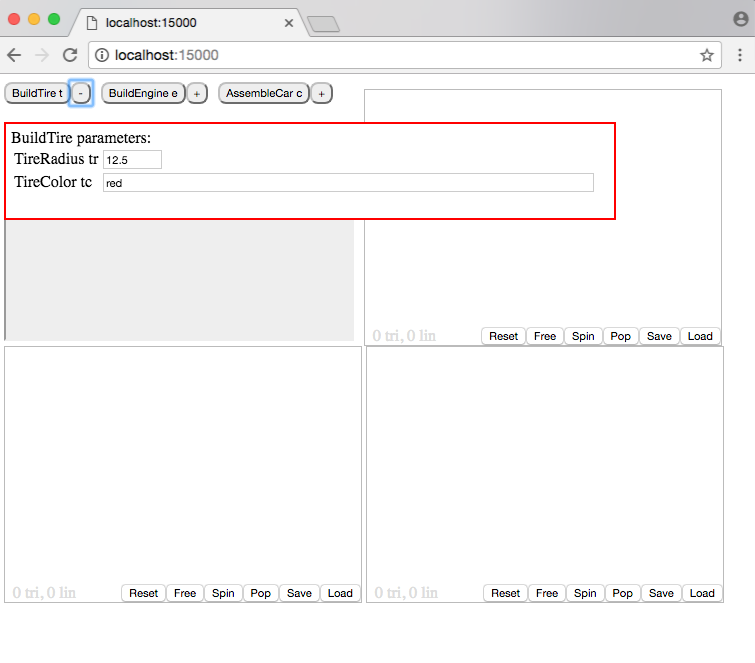
\includegraphics[width=0.75\textwidth]{pix/buttons.png}
\caption{\f{WEBGUI} after calling \textbf{webinit} to create 3 command buttons and store 4 parameters. In this picture,
the user has toggled the drop down menu for BuildTire revealing 2 parameters.}
\label{fig:3}
\end{figure}

%%%%%%%%%%%%%%%%%%%%%%%%%%%%%%%%%%%%%%%%%%%%%%%%%%%%%%%%%%%%%%%%%%%%%%%%%%%%
% WEBUPDATE
%%%%%%%%%%%%%%%%%%%%%%%%%%%%%%%%%%%%%%%%%%%%%%%%%%%%%%%%%%%%%%%%%%%%%%%%%%%%
\newpage
\subsection{webupdate}
\underline{Description} The function \textbf{void webupdate(int* ip, double* rp, char* sp)} updates (changes)
the parameters being stored in the web browser GUI. By default, the web browser GUI doesn't store any parameters,
but by using \textbf{webinit}, you can have the GUI store variables (so the user can view and change them).
The function \textbf{webupdate} can be called anytime after \textbf{webinit} (and before or after \textbf{webstart}). Read
Section \ref{sec:3-4} to learn more about parameters and updating them.\\
\\
\underline{Declaration}
\begin{verbatim} 
	void webupdate(int* ip, double* rp, char* sp)
\end{verbatim}
\underline{Parameters}\\
\textbf{ip} is an array of (4 byte) integers. If your web browser GUI is storing integer parameters (as a result of
a previous call to \textbf{webinit}), they will be updated to these values.\\
\textbf{rp} is an array of (8 byte) doubles. If your web browser GUI is storing double parameters (as a result of
a previous call to \textbf{webinit}), they will be updated to these values.\\
\textbf{sp} is an array of strings of length 80. If your web browser GUI is storing string parameters (as a result of
a previous call to \textbf{webinit}), they will be updated to these values. These strings can be
either null terminated as is the convention of C strings or they can be padded with spaces as is the convenction
of Fortran strings. However, the second string must start at str[80], and the third string at str[160], etc. Therefore,
be careful if you use \textbf{malloc} in C. Make sure to allocate a contiguous block of memory.\\
\\
\underline{Example} The following example shows the usage of \textbf{webupdate}.
\begin{verbatim}
#include <webgui.h>
#include <unistd.h>

int main(){
    char str[14][80] = {
        "c c=BuildTire, k=t",
        "c c=BuildEngine, k=e",
        "c c=AssembleCar, k=c",
        "n n=TireRadius, a=tr, t=r, i=1, d=12.5",
        "n n=TireColor, a=tc, t=s, i=1, d=red",
        "n n=EngineSize, a=es, t=i, i=1, d=300",
        "n n=CarColor, a=cc, t=i, i=2, d=1",
        "r c=BuildTire, n=TireRadius",
        "r c=BuildTire, n=TireColor",
        "r c=BuildEngine, n=EngineSize",
        "r c=AssembleCar, n=CarColor",
        "s n=CarColor, v=0, l=red",
        "s n=CarColor, v=1, l=white",
        "s n=CarColor, v=2, l=blue"
    };
    int ip[2] = {400,2};
    double rp[1] = {13.5};
    char sp[1][80] = {"black"};
    webinit((char*)str,14);
    webstart(15000);
    webupdate(ip,rp,(char*)sp);
    pause();
    return 0;
}
\end{verbatim}
After compiling and running the above program, initially the parameter values of TireRadius, TireColor, EngineSize,
and CarColor are set to 12.5, red, 300, and 1 respectively. The call to \textbf{webupddate} changes these values
to 13.5, black, 400, and 2 respectively.
\begin{figure}[b!]
\centering
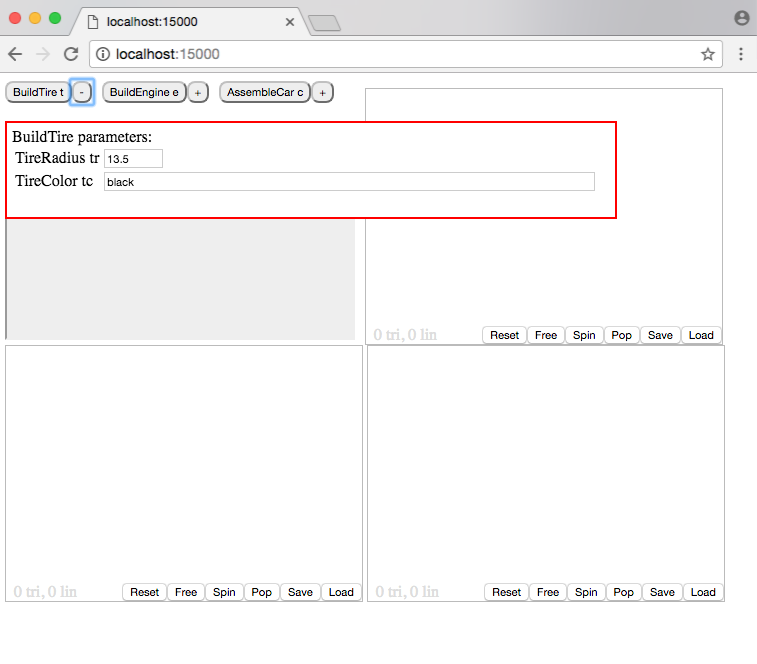
\includegraphics[width=0.75\textwidth]{pix/buttons2.png}
\caption{\f{WEBGUI} after calling \textbf{webinit} and then \textbf{webupdate}. Parameter values TireRadius and TireColor
changed from 12.5 and red to 13.5 and black.}
\label{fig:4}
\end{figure}

%%%%%%%%%%%%%%%%%%%%%%%%%%%%%%%%%%%%%%%%%%%%%%%%%%%%%%%%%%%%%%%%%%%%%%%%%%%%
% WEBSETTITLE
%%%%%%%%%%%%%%%%%%%%%%%%%%%%%%%%%%%%%%%%%%%%%%%%%%%%%%%%%%%%%%%%%%%%%%%%%%%%
\newpage
\subsection{websettitle}
\underline{Description} The function \textbf{void websettitle(char* str)} is called before \textbf{webstart} if the user wishes for the web browser GUI's
webpage to show a title on top of the web browser.\\
\\
\underline{Declaration}
\begin{verbatim} 
	void websettitle(char* str)
\end{verbatim}
\underline{Parameters} \textbf{str} is a string of length 80 or less. This string can either be null terminated as is the convention 
of C strings, or the unused characters of the array length should be filled with spaces as is the convention of Fortran strings.\\
\\
\underline{Example} The following example shows the usage of \textbf{webwriteline}.
\begin{verbatim}
#include <webgui.h>
#include <unistd.h>

int main(){
    websettitle("Sample program");
    webstart(15000);
    pause();
    return 0;
}
\end{verbatim}
After compiling and running the above program, the web browser's webpage will show the title, "Sample program".

%%%%%%%%%%%%%%%%%%%%%%%%%%%%%%%%%%%%%%%%%%%%%%%%%%%%%%%%%%%%%%%%%%%%%%%%%%%%
% WEBSTOP
%%%%%%%%%%%%%%%%%%%%%%%%%%%%%%%%%%%%%%%%%%%%%%%%%%%%%%%%%%%%%%%%%%%%%%%%%%%%
\subsection{webstop}
\underline{Description} The function \textbf{void webstop()} terminates the web server. Afterward web browsers can no longer
connect and display the graphical interface. Also, the listening thread is terminated and all memory is freed.\\
\\
\underline{Declaration} 
\begin{verbatim} 
	void webstop()
\end{verbatim}


\newpage
\section{2D Image display}
\label{sec:2-3}
%%%%%%%%%%%%%%%%%%%%%%%%%%%%%%%%%%%%%%%%%%%%%%%%%%%%%%%%%%%%%%%%%%%%%%%%%%%%
% WEBSETCOLORS
%%%%%%%%%%%%%%%%%%%%%%%%%%%%%%%%%%%%%%%%%%%%%%%%%%%%%%%%%%%%%%%%%%%%%%%%%%%%
\subsection{websetcolors}
\underline{Description} The function \textbf{void websetcolors(int nc, double* R, double* G, double* B, int pane)} 
defines a color palette to be used by subsequent calls. Colors are defined by giving their red, green, blue amounts.
This function defines a color palette for one of the three display panes. Each pane has two palettes; one for 2D images and
one for 3D objects. Call this function before sending any information about
2D images with \textbf{webimagedisplay} and before sending any information about 3D objects with \textbf{webline} and
\textbf{webfill}.\\
\\
\underline{Declaration} 
\begin{verbatim} 
    void websetcolors(int nc, double* R, double* G, double* B, int pane)
\end{verbatim}
\underline{Parameters} \textbf{nc} is a (4 byte) integer stating the number of colors in the palette. 
For 2D images, the maximum value of \textbf{nc} is 256. (For 3D objects, max is 2 billion.)\\
\textbf{R} is an array of (8 byte) doubles. The length of the array is \textbf{nc}. The first element of this array
is the amount of red in the first color. The value of each element should be between 0.0 and 1.0 inclusive.\\
\textbf{G} is an array of (8 byte) doubles. The length of the array is \textbf{nc}. The first element of this array
is the amount of green in the first color.  The value of each element should be between 0.0 and 1.0 inclusive.\\
\textbf{B} is an array of (8 byte) doubles. The length of the array is \textbf{nc}. The first element of this array
is the amount of blue in the first color.  The value of each element should be between 0.0 and 1.0 inclusive.\\
\textbf{pane} is a (4 byte) integer stating which display pane's color palette you are defining. Use integers
0, 1, 2 to define palettes for 3D objects corresponding with panes top right, bottom left, and bottom right respectively. 
Use 3, 4, 5 to define the color palette's for 2D images corresponding with panes top right, bottom left, and bottom 
right respectively.\\
\\
\underline{Example} The following example shows the usage of \textbf{websetcolors}. Imagine that you would like
to define and later use the 6 colors of the rainbow. In conventional RGB, red is RGB = (255,0,0); orange is 
RGB = (255,128,0); yellow is RGB = (255,255,0); green is RGB = (0,255,0); blue is RGB = (0,0,255); and purple
is RGB = (128,0,128). The follow code defines this palette for a 2D image in pane 3.
\begin{verbatim}
double red[6] = {1.0, 1.0, 1.0, 0.0, 0.0, 0.5};
double green[6] = {0.0, 0.5, 1.0, 1.0, 0.0, 0.0};
double blue[6] = {0.0, 0.0, 0.0, 0.0, 1.0, 0.5};
websetcolors(6,red,green,blue,3); 
\end{verbatim}
This program defines a color palette with the 6 colors of the rainbow for 2D images in pane 3. Subsequent calls to 
\textbf{webimagedisplay} in the top right display pane will use this color palette.

%%%%%%%%%%%%%%%%%%%%%%%%%%%%%%%%%%%%%%%%%%%%%%%%%%%%%%%%%%%%%%%%%%%%%%%%%%%%
% WEBIMAGEDISPLAY
%%%%%%%%%%%%%%%%%%%%%%%%%%%%%%%%%%%%%%%%%%%%%%%%%%%%%%%%%%%%%%%%%%%%%%%%%%%%
\newpage
\subsection{webimagedisplay}
\underline{Description} The function \textbf{void webimagedisplay(int nx, int ny, int* image, int pane)} displays a
2D image in the designated display pane. Before calling this, you must call \textbf{websetcolors} to define a palette
to be referenced.\\
\\
\underline{Declaration}
\begin{verbatim}
void webimagedisplay(int nx, int ny, int* image, int pane)
\end{verbatim}
\underline{Parameters} \textbf{nx} is a (4 byte) integer stating the pixel width of the image to be displayed. The
variable \textbf{nx} must be divisible by 4.\\
\textbf{ny} is a (4 byte) integer stating the pixel height of the image to be displayed.\\
\textbf{image} is an array of (4 byte) integers of size \textbf{nx} width and \textbf{ny} height. Each integer represents
a pixel. Each integer's value is between and including 0 and \textbf{nc}-1, the number of colors in the palette you previously 
declared by calling \textbf{websetcolors}. Note that the first color in your palette is referred to as 0 not 1. The second 
color is 1, not 2, etc. The variable \textbf{image} is assumed to reside in memory contiguously row by row as is the 
convention in C. Fortran stores arrays column by column so you need to be careful. Furthermore, the image is drawn 
row by row from the bottom upward.  So your array's first row of integers 
will be the bottom row of your image and your array's last row of integers will be the top row of your image. 
Also note that your image will display in a rectangle with aspect ratio 1.5 width by 1.0 height. (Therefore it looks best
if $nx = 1.5 ny$. This is optional not mandatory.) See example below.\\
\textbf{pane} is a (4 byte) integer stating which display pane to display the image in. Valid integers are 3, 4, 5. These
refer to the top right, bottom left, and bottom right display panes respectively. Note that this integer should match the 
integer that you used to set the palette with \textbf{websetcolors}. \\
\\
\underline{Example} The following example shows the usage of \textbf{webimagedisplay} in the C programming language.
\begin{verbatim}
double red[7] = {1.0, 1.0, 1.0, 0.0, 0.0, 0.5, 0.0};
double green[7] = {0.0, 0.5, 1.0, 1.0, 0.0, 0.0, 0.0};
double blue[7] = {0.0, 0.0, 0.0, 0.0, 1.0, 0.5, 0.0};
websetcolors(7,red,green,blue,3); 
int image[6][4] = { 
    {0,0,0,6},
    {1,1,1,6}, 
    {2,2,2,6}, 
    {3,3,3,6}, 
    {4,4,4,6},
    {5,5,5,6}
};
webimagedisplay(4,6,image,3);
\end{verbatim}
After this program is compiled and ran, it will display an image in the top right display pane as show in Figure \ref{fig:5}.
The first call to \textbf{websetcolors} defines a 2D image palette in pane 3 with colors 0, 1, 2, 3, 4, 5, 6 being red, orange, yellow, green, 
blue, purple, black respectively. The second call to \textbf{webimagedisplay} defines and draws the image.
Notice how the first row of "0,0,0,6" which refers to colors red, red, red, black is the bottom row of the image and the last
row "5,5,5,6" which refers to colors purple, purple, purple, black is the first row of the image. This is illustrated in Figure \ref{fig:6}.

Note that Fortran places arrays of integers in memory contiguously column by column. Therefore to display this same image 
in Fortran, the code would be:

\begin{verbatim}
integer(kind=4), dimension(4,6) :: image
real(kind=8), dimension(7) :: red,green,blue
data r/1.0,1.0,1.0,0.0,0.0,0.5,0.0/
data g/0.0,0.5,1.0,1.0,0.0,0.0,0.0/
data b/0.0,0.0,0.0,0.0,1.0,0.5,0.0/
do j=1,6
    do i=1,3
        image(i,j)=j-1
    enddo
    image(4,j)=6
enddo
call websetcolors(7,red,green,blue,3)
call webimagedisplay(4,6,image,3)
\end{verbatim}

or you could force Fortran to place rows together in memory by writing this:

\begin{verbatim}
integer(kind=4), dimension(24) :: image
do i=0,5
    do j=1,3
        image(4*i+j)=i
    enddo
    image(4*i+4)=6
enddo
call websetcolors(7,red,green,blue,3)
call webimagedisplay(4,6,image,3)
\end{verbatim}

Another example of using \textbf{webimagedisplay} can be found in Section \ref{sec:2-11}. See example 2.

\newpage
\begin{figure}[H]
\centering
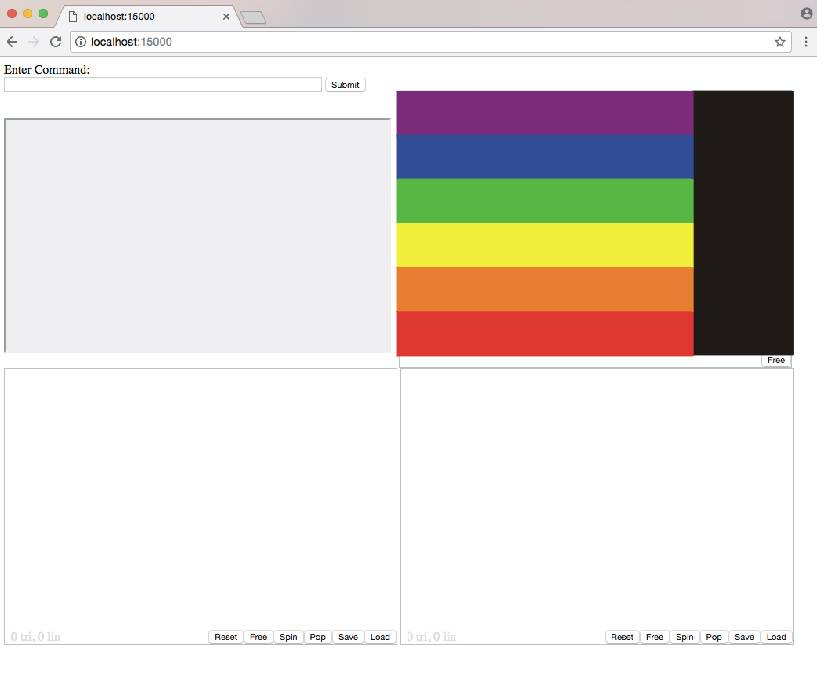
\includegraphics[width=0.75\textwidth]{pix/image2.jpg}
\caption{\f{WEBGUI} after calling \textbf{websetcolors} and \textbf{webimagedisplay}.}
\label{fig:5}
\end{figure} 

\begin{figure}[H]
\centering
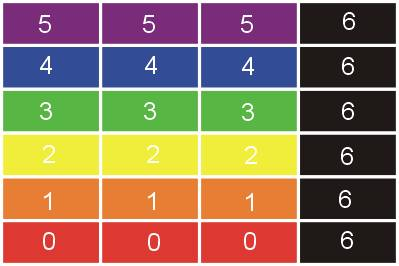
\includegraphics[width=0.75\textwidth]{pix/image3.jpg}
\caption{How the \textbf{image} array becomes an image.}
\label{fig:6}
\end{figure}
 
\newpage
\section{3D Object display}
\label{sec:2-4}
%%%%%%%%%%%%%%%%%%%%%%%%%%%%%%%%%%%%%%%%%%%%%%%%%%%%%%%%%%%%%%%%%%%%%%%%%%%%
% WEBSETCOLORS
%%%%%%%%%%%%%%%%%%%%%%%%%%%%%%%%%%%%%%%%%%%%%%%%%%%%%%%%%%%%%%%%%%%%%%%%%%%%
\subsection{websetcolors}
\underline{Description} The function \textbf{void websetcolors(int nc, double* R, double* G, double* B, int pane)} 
defines a color palette to be used by subsequent calls. Colors are defined by giving their red, green, blue amounts.
This function defines a color palette for one of the three display panes. Each pane has two palettes; one for 2D images and
one for 3D objects. Call this function before sending any information about
2D images with \textbf{webimagedisplay} and before sending any information about 3D objects with \textbf{webline} and
\textbf{webfill}.\\
\\
\underline{Declaration} 
\begin{verbatim} 
    void websetcolors(int nc, double* R, double* G, double* B, int pane)
\end{verbatim}
\underline{Parameters} \textbf{nc} is a (4 byte) integer stating the number of colors in the palette.\\
\textbf{R} is an array of (8 byte) doubles. The length of the array is \textbf{nc}. The first element of this array
is the amount of red in the first color. The value of each element should be between 0.0 and 1.0 inclusive.\\
\textbf{G} is an array of (8 byte) doubles. The length of the array is \textbf{nc}. The first element of this array
is the amount of green in the first color.  The value of each element should be between 0.0 and 1.0 inclusive.\\
\textbf{B} is an array of (8 byte) doubles. The length of the array is \textbf{nc}. The first element of this array
is the amount of blue in the first color.  The value of each element should be between 0.0 and 1.0 inclusive.\\
\textbf{pane} is a (4 byte) integer stating which display pane's color palette you are defining. Use integers
0, 1, 2 to define palettes for 3D objects corresponding with panes top right, bottom left, and bottom right respectively. 
Use 3, 4, 5 to define the color palette's for 2D images corresponding with panes top right, bottom left, and bottom 
right respectively.\\
\\
\underline{Example} The following example shows the usage of \textbf{websetcolors}. Imagine that you would like
to define and later use the 6 colors of the rainbow. In conventional RGB, red is RGB = (255,0,0); orange is 
RGB = (255,128,0); yellow is RGB = (255,255,0); green is RGB = (0,255,0); blue is RGB = (0,0,255); and purple
is RGB = (128,0,128). The follow code defines this palette for a 2D image in pane 3.
\begin{verbatim}
double red[6] = {1.0, 1.0, 1.0, 0.0, 0.0, 0.5};
double green[6] = {0.0, 0.5, 1.0, 1.0, 0.0, 0.0};
double blue[6] = {0.0, 0.0, 0.0, 0.0, 1.0, 0.5};
websetcolors(6,red,green,blue,3); 
\end{verbatim}
This program defines a color palette with the 6 colors of the rainbow for 2D images in pane 3. Subsequent calls to 
\textbf{webimagedisplay} in the top right display pane will use this color palette.

%%%%%%%%%%%%%%%%%%%%%%%%%%%%%%%%%%%%%%%%%%%%%%%%%%%%%%%%%%%%%%%%%%%%%%%%%%%%
% WEBFRAME
%%%%%%%%%%%%%%%%%%%%%%%%%%%%%%%%%%%%%%%%%%%%%%%%%%%%%%%%%%%%%%%%%%%%%%%%%%%%
\newpage
\subsection{webframe}
\label{sec:2-12}
\underline{Description} The function \textbf{void webframe(int frame)} declares which portion of a display pane subsequent 
calls to \textbf{webline} and \textbf{webfill} will draw in. The web browser GUI has 3 display panes and each display pane is divided
into 3 frames (or sub panes). Call this function after \textbf{websetcolors} and before drawing lines and polygons with \textbf{webline} 
and \textbf{webfill}. Note that to draw multiple lines and polygons in a particular frame, you only need to call \textbf{webframe} once and 
then follow with multiple calls to \textbf{webline} and \textbf{webfill}.\\
\\
\underline{Declaration}
\begin{verbatim}
void webframe(int frame)
\end{verbatim}
\underline{Parameters} \textbf{frame} is a (4 byte) integer stating which frame to draw future calls to \textbf{webline} and \textbf{webfill} in.
Valid integers are 1, 2, 3, 4, 5. Each display pane is a rectangle with aspect ratio width to height as 1.5 to 1.0. This rectangle is the 
union of 3 squares, see Figure \ref{fig:10}. The big square on the left is $frame = 4$, the square in the top right is $frame = 2$, and the square
in the bottom right is $frame = 3$. After declaring a frame, all subsequent calls will draw in this square only. After drawing to frames 2, 3, 4,
the resultant 3D objects will not be able to be zoomed, panned, nor rotated. If you wish for your object to be zoomed, panned, and rotated
then draw to $frame = 5$. Frame 5 draws to the big square on the left ($frame=4$) but provides the ability of zoom, pan, and rotate. Lastly,
set $frame=1$ if you wish to draw to the entire rectangle display pane ignoring the sub pane structure.\\
\\
\underline{Example} To see an example of \textbf{webframe}, read the example in the next subsection \ref{sec:2-5}, \textbf{webline}.

\begin{figure}[H]
\centering
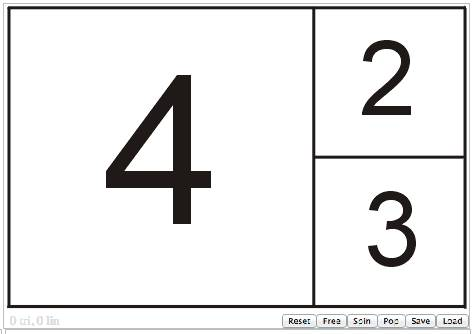
\includegraphics[width=0.75\textwidth]{pix/frame.jpg}
\caption{Frames 2, 3, 4 within a display pane.}
\label{fig:10}
\end{figure} 

%%%%%%%%%%%%%%%%%%%%%%%%%%%%%%%%%%%%%%%%%%%%%%%%%%%%%%%%%%%%%%%%%%%%%%%%%%%%
% WEBLINEFLT
%%%%%%%%%%%%%%%%%%%%%%%%%%%%%%%%%%%%%%%%%%%%%%%%%%%%%%%%%%%%%%%%%%%%%%%%%%%%
\newpage
\subsection{weblineflt}
\label{sec:2-5}
\underline{Description} The function \textbf{void weblineflt(float* x, float* y, float* z, int n, int color)} draws a line in the display pane
that was last declared with \textbf{websetcolors} using the colors declared in \textbf{websetcolors} and within the sub pane (frame)
declared with the last call to \textbf{webframe}.\\
\\
\underline{Declaration}
\begin{verbatim}
void weblineflt(float* x, float* y, float* z, int n, int color)
\end{verbatim}
\underline{Parameters} \textbf{x, y, z} are arrays of (4 byte) single precision floating point real numbers. The first number in each array
are the $x,y,z$ coordinates of your first point in 3D. The second elements are the second point, etc. You can submit any number of points 
and this function draws line segments between each consecutive pair of points. The values of \textbf{x,y,z} are between 0.0 and 1.0 inclusive.
The center of each frame (sub pane) is $(x,y,z)=(0.5,0.5,0.5)$, the bottom left corner is $(x,y,z)=(0,0,z)$ and the top right corner is $(x,y,z)=(1,1,z)$.
Positive \textbf{z} comes out of the screen, while negative \textbf{z} goes into the screen.
An exception to these bounds is $frame = 1$ which accesses the entire display pane rectangle. 
In this case the value of \textbf{x} is between 0.0 and 1.5 inclusive. (and \textbf{y} is still between 0.0 and 1.0). The 
bottom left corner is $(x,y,z)=(0,0,z)$ and the top right corner is $(x,y,z)=(1.5,1,z)$.\\
\textbf{n} is a (4 byte) integer stating the length of arrays \textbf{x,y,z} which is the number of 3D points that your are submitting.\\
\textbf{color} is a (4 byte) integer between 1 and \textbf{nc}, where \textbf{nc} is the number of colors you declared in your last call
to \textbf{websetcolors}. The value \textbf{color} references those colors with 1 being the first color (not 0), 2 the second (not 1), etc. 
All line segments will be drawn with this color.\\
\\
\underline{Example} The following example shows the usage of \textbf{weblineflt}.
\begin{verbatim}
double red[3]={1.0,0.0,0.0};
double green[3]={0.0,1.0,0.0};
double blue[3]={0.0,0.0,1.0};
websetcolors(3,red,green,blue,0);
float x[4]={0.0,0.75,0.5,0.0};
float y[4]={0.0,0.25,0.75,0.0};
float z[4]={0.5,0.5,0.5,0.0};
webframe(4);
weblineflt(x,y,z,4,1);
webframe(3);
weblineflt(x,y,z,4,2);
webframe(2);
weblineflt(x,y,z,4,3);
webgldisplay(0);
\end{verbatim}
The above block of code, defines a 3D object color palette for display pane 0 (top right pane) declaring the 3 colors red, green, blue as a result of the first call to 
\textbf{websetcolors}. Furthermore, \textbf{websetcolors} declares that subsequent calls to \textbf{webline} and \textbf{webfill} will draw lines and polygons 
in display pane 0. The first call to \textbf{webframe} declares future drawing to be in the sub pane of $frame=4$. The subsequent call to \textbf{weblineflt} draws a 
triangle of $color=1$ which is red into $frame=4$ of $pane=0$. A second call to \textbf{webframe} and \textbf{weblineflt} draws a triangle of  $color=2$ 
which is green into $frame=2$ of $pane=0$. And a third call to  \textbf{webframe} and \textbf{weblineflt} draws a triangle of $color=3$ which is blue into 
$frame=3$ of $pane=0$. Lastly, calling \textbf{webgldisplay} displays the 3D object in display pane 0. See Figure \ref{fig:8}.

\begin{figure}[H]
\centering
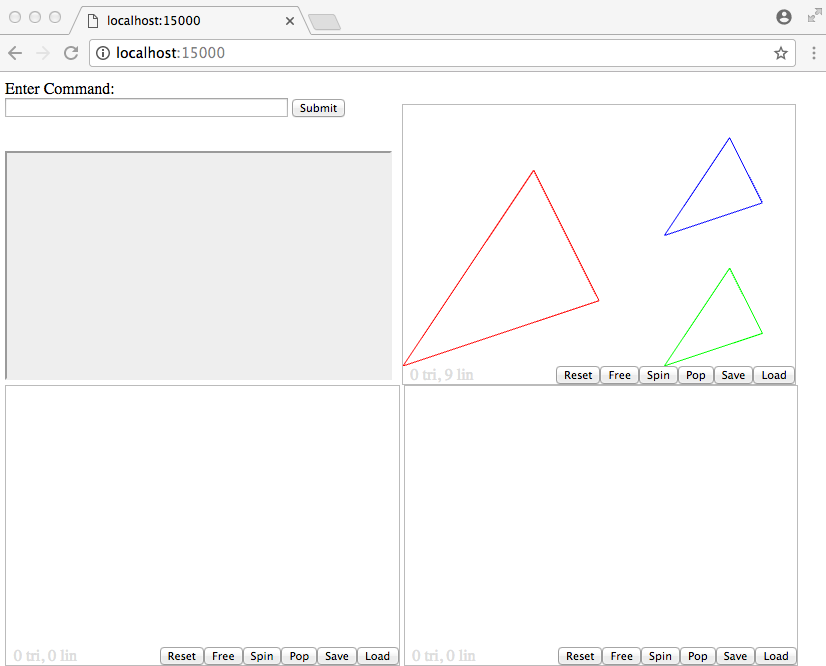
\includegraphics[width=0.75\textwidth]{pix/lines.png}
\caption{\f{WEBGUI} after calling \textbf{webline} three times in display pane 0 with different frames and colors.}
\label{fig:8}
\end{figure} 

Below is another example. It draws a black triangle in $frame=1$ of $pane=1$. Output shown in Figure \ref{fig:9}.
\begin{verbatim}
double red[1]={0.0};
double green[1]={0.0};
double blue[1]={0.0};
websetcolors(1,red,green,blue,1);
float x[4]={0.0,1.5,0.25,0.0};
float y[4]={0.75,0.25,0.25,0.75};
float z[4]={0.5,0.5,0.5,0.5};
webframe(1);
weblineflt(x,y,z,4,1);
webgldisplay(1);
\end{verbatim}
\begin{figure}[H]
\centering
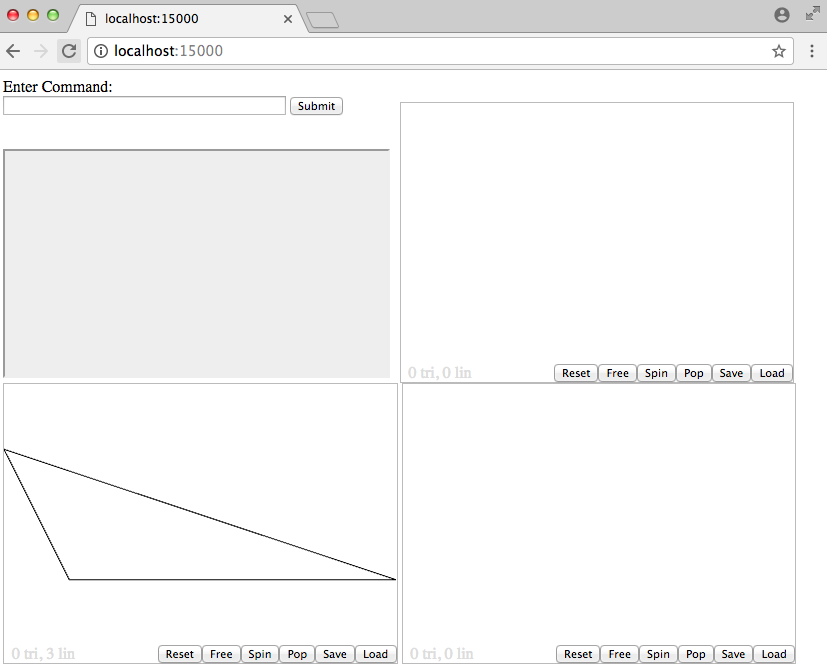
\includegraphics[width=0.75\textwidth]{pix/lines2.png}
\caption{\f{WEBGUI} after calling \textbf{webframe(1)} and \textbf{webline} in display pane 1.}
\label{fig:9}
\end{figure}

%%%%%%%%%%%%%%%%%%%%%%%%%%%%%%%%%%%%%%%%%%%%%%%%%%%%%%%%%%%%%%%%%%%%%%%%%%%%
% WEBFILLFLT
%%%%%%%%%%%%%%%%%%%%%%%%%%%%%%%%%%%%%%%%%%%%%%%%%%%%%%%%%%%%%%%%%%%%%%%%%%%%
\newpage
\subsection{webfillflt}
\label{sec:2-6}
\underline{Description} The function \textbf{void webfillflt(float* x, float* y, float* z, int n, int color)} draws a filled convex polygon in the display pane
that was last declared with \textbf{websetcolors} using the colors declared in \textbf{websetcolors} and within the sub pane (frame)
declared with the last call to \textbf{webframe}.\\
\\
\underline{Declaration}
\begin{verbatim}
void webfillflt(float* x, float* y, float* z, int n, int color)
\end{verbatim}
\underline{Parameters} \textbf{x, y, z} are arrays of (4 byte) single precision floating point real numbers. The first number in each array
are the $x,y,z$ coordinates of your first vertex in 3D. The second elements are the second vertex, etc. You can submit any number of vertices 
and this function draws filled triangles between each consecutive pair of vertices together with the first vertex (thus drawing the entire filled convex polygon). 
The values of \textbf{x,y,z} are between 0.0 and 1.0 inclusive.
The center of each frame (sub pane) is $(x,y,z)=(0.5,0.5,0.5)$, the bottom left corner is $(x,y,z)=(0,0,z)$ and the top right corner is $(x,y,z)=(1,1,z)$.
Positive \textbf{z} comes out of the screen, while negative \textbf{z} goes into the screen.
An exception to these bounds is $frame = 1$ which accesses the entire display pane rectangle. 
In this case the value of \textbf{x} is between 0.0 and 1.5 inclusive. (and \textbf{y} is still between 0.0 and 1.0). The 
bottom left corner is $(x,y,z)=(0,0,z)$ and the top right corner is $(x,y,z)=(1.5,1,z)$.\\
\textbf{n} is a (4 byte) integer stating the length of arrays \textbf{x,y,z} which is the number of 3D vertices that your are submitting.\\
\textbf{color} is a (4 byte) integer between 1 and \textbf{nc}, where \textbf{nc} is the number of colors you declared in your last call
to \textbf{websetcolors}. The value \textbf{color} references those colors with 1 being the first color (not 0), 2 the second (not 1), etc. 
The entire filled polygon (all separate triangles) will be drawn with this color.\\
\\
\underline{Example} The following example shows the usage of \textbf{webfillflt}.
\begin{verbatim}
double red[3] = {1.0, 1.0, 1.0};
double green[3] = {0.0, 0.5, 1.0};
double blue[3] = {0.0, 0.0, 0.0};
websetcolors(3,red,green,blue,0);
webframe(5);
float xA[5]={0.25,0.75,0.75,0.25,0.25};
float yA[5]={0.25,0.25,0.75,0.75,0.25};
float zA[5]={0.75,0.75,0.75,0.75,0.75};
webfillflt(xA,yA,zA,5,1);
float xB[5]={0.25,0.75,0.75,0.25,0.25};
float yB[5]={0.25,0.25,0.25,0.25,0.25};
float zB[5]={0.25,0.25,0.75,0.75,0.25};
webfillflt(xB,yB,zB,5,2);
float xC[5]={0.25,0.25,0.25,0.25,0.25};
float yC[5]={0.25,0.75,0.75,0.25,0.25};
float zC[5]={0.25,0.25,0.75,0.75,0.25};
webfillflt(xC,yC,zC,5,3);
webgldisplay(0);
\end{verbatim}
The above block of code, defines a 3D object color palette for display pane 0 (top right pane) declaring the 3 colors red, orange, yellow as a result of the first call to 
\textbf{websetcolors}. Furthermore, \textbf{websetcolors} declares that subsequent calls to \textbf{webline} and \textbf{webfill} will draw lines and polygons 
in display pane 0. Then \textbf{webframe} declares future drawing to be in the sub pane of $frame=5$. The subsequent call to \textbf{webfillflt} draws one
face of a cube (a square) with $color=1$ which is red into $frame=5$ of $pane=0$. A second call to \textbf{webframe} and \textbf{webfillflt} draws a second face of a cube
with $color=2$ which is orange into $frame=5$ of $pane=0$. And a third call to  \textbf{webframe} and \textbf{webfillflt} draws a third face of a cube with $color=3$ 
which is yellow into $frame=5$ of $pane=0$. Lastly, calling \textbf{webgldisplay} displays the 3D object in display pane 0. After the 3D object is displayed,
the user can rotate the cube so that one vertex is pointed forward. See Figure \ref{fig:11}.
\begin{figure}[H]
\centering
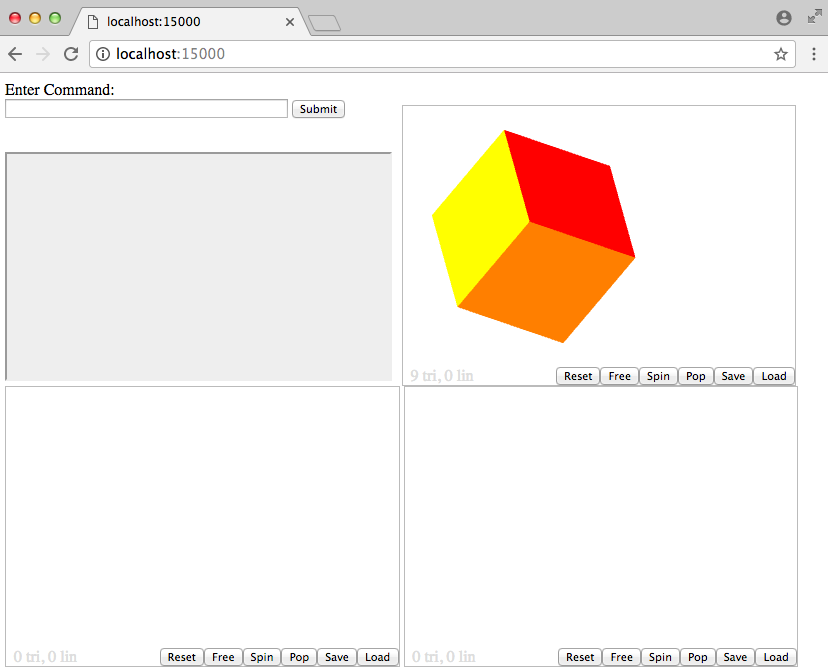
\includegraphics[width=0.75\textwidth]{pix/cube.png}
\caption{\f{WEBGUI} after calling \textbf{webfill} three times in display pane 0 and rotating the object.}
\label{fig:11}
\end{figure} 

%%%%%%%%%%%%%%%%%%%%%%%%%%%%%%%%%%%%%%%%%%%%%%%%%%%%%%%%%%%%%%%%%%%%%%%%%%%%
% WEBLINEDBL and FILLDBL
%%%%%%%%%%%%%%%%%%%%%%%%%%%%%%%%%%%%%%%%%%%%%%%%%%%%%%%%%%%%%%%%%%%%%%%%%%%%
\newpage
\subsection{weblinedbl}
\underline{Description} The function \textbf{void weblinedbl(double* x, double* y, double* z, int n, int color)} is the same as \textbf{weblineflt} 
except that the array arguments are double precision reals instead of single precision. Note that \f{WEBGUI} only draws lines in single 
precision, but you should call either \textbf{weblineflt} or \textbf{weblinedbl} based on how your vertices are stored in your software either as single 
precision (4 byte reals) or double precision (8 byte reals). Don't cast your variables, let \f{WEBGUI} do the casting for you.\\
\\
\subsection{webfilldbl}
\underline{Description} The function \textbf{void webfilldbl(double* x, double* y, double* z, int n, int color)} is the same as \textbf{webfillflt} 
except that the array arguments are double precision reals instead of single precision. Note that \f{WEBGUI} only draws triangles in single 
precision, but you should call either \textbf{weblineflt} or \textbf{weblinedbl} based on how your vertices are stored in your software either as single 
precision (4 byte reals) or double precision (8 byte reals). Don't cast your variables, let \f{WEBGUI} do the casting for you.\\
\\
\subsection{webgldisplay}
\underline{Description} The function \textbf{void webgldisplay(int pane)} displays the 3D object that was previously sent to the indicated display 
pane. Call this function after calling \textbf{websetcolors}, \textbf{webframe}, \textbf{webline}, and \textbf{webfill}.\\
\\
\underline{Declaration}
\begin{verbatim}
void webgldisplay(int pane)
\end{verbatim}
\underline{Parameters} \textbf{pane} is a (4 byte) integer stating which display pane should display its 3D object. Valid integers are 0, 1, 2 
referring to the top right, bottom left, and bottom right display pane. The variable \textbf{pane} should match the value in your previous call
to \textbf{websetcolors}.\\
\\
\underline{Example} For an example of \textbf{webgldisplay}, see the examples in the previous sub sections, \ref{sec:2-5} and \ref{sec:2-6}.

\newpage
\section{Miscellaneous}

%%%%%%%%%%%%%%%%%%%%%%%%%%%%%%%%%%%%%%%%%%%%%%%%%%%%%%%%%%%%%%%%%%%%%%%%%%%%
% WEBQUERY
%%%%%%%%%%%%%%%%%%%%%%%%%%%%%%%%%%%%%%%%%%%%%%%%%%%%%%%%%%%%%%%%%%%%%%%%%%%%
\subsection{webquery}
\underline{Description} The function \textbf{int webquery()} informs the caller whether the web browser is displaying command buttons or not. Even 
if your software calls \textbf{webinit} to create command buttons, the user can toggle them off and on with key strokes, therefore this function exists. 
(To learn how to toggle buttons off and on, see Section \ref{sec:4-1})\\
\\
\underline{Declaration}
\begin{verbatim}
int webquery()
\end{verbatim}
\underline{Return Value} If command buttons are showing, 1 is returned. If a command prompt to accept only typed strings is showing, 0 is returned.
\\
%%%%%%%%%%%%%%%%%%%%%%%%%%%%%%%%%%%%%%%%%%%%%%%%%%%%%%%%%%%%%%%%%%%%%%%%%%%%
% WEBBUTTON
%%%%%%%%%%%%%%%%%%%%%%%%%%%%%%%%%%%%%%%%%%%%%%%%%%%%%%%%%%%%%%%%%%%%%%%%%%%%
\subsection{webbutton}
\underline{Description} The function \textbf{void webbutton(int highlight, char* cmd)} will highlight a command button by making it a darker gray. This
is a useful function to indicate whether a feature of your software is turned on or off.\\
\\
\underline{Declaration}
\begin{verbatim}
void webbutton(int highlight, char* cmd)
\end{verbatim}
\underline{Parameters} \textbf{highlight} is a (4 byte) integer of value 1 or 0. Setting $highlight=1$, causes the indicated command button to be 
highlighted. Setting $highlight=0$ causes the indicated command button to be unhighlighted (normal).\\
\textbf{cmd} is a string of length 20 or less. \textbf{cmd} can be either a NULL terminated C type string, or it can be a Fortran type
string padded with spaces to its array length. The string \textbf{cmd} must match the command name that you supplied in \textbf{webinit} (with
the key value pair associated with c.)\\
\\
%%%%%%%%%%%%%%%%%%%%%%%%%%%%%%%%%%%%%%%%%%%%%%%%%%%%%%%%%%%%%%%%%%%%%%%%%%%%
% WEBPAUSE
%%%%%%%%%%%%%%%%%%%%%%%%%%%%%%%%%%%%%%%%%%%%%%%%%%%%%%%%%%%%%%%%%%%%%%%%%%%%
\subsection{webpause}
\underline{Description} The function \textbf{void webpause()} requests that the user click a continue button before proceeding. This is useful if your 
software is outputting multiple images that potentially overwrite themselves. You can request the user click continue which forces them to view the
image before proceeding.
\\
\underline{Declaration}
\begin{verbatim}
void webpause()
\end{verbatim}

%%%%%%%%%%%%%%%%%%%%%%%%%%%%%%%%%%%%%%%%%%%%%%%%%%%%%%%%%%%%%%%%%%%%%%%%%%%%
% WEBSETMODE
%%%%%%%%%%%%%%%%%%%%%%%%%%%%%%%%%%%%%%%%%%%%%%%%%%%%%%%%%%%%%%%%%%%%%%%%%%%%
\newpage
\subsection{websetmode}
\label{sec:2-11}
\underline{Description} The function \textbf{void websetmode(int x)} can allow your program to receive the keyboard and mouse presses from
the web browser. It can also allow your program to display 2D images or 3D objects faster than the default two per second (thus simulating 
animation). And this function determines whether new 3D objects inherit zoom, pan, and rotation settings from previously displayed 3D objects. 
By default, \f{WEBGUI} runs in mode 0. If this is adequate, you do not need to call \textbf{websetmode}. 
This function can be called as often as you like and before or after \textbf{webstart}. Recommended usage is to change the mode when needed 
and change back to 0 when not needed.\\
\\
\underline{Declaration}
\begin{verbatim}
void websetmode(int x)
\end{verbatim}
\underline{Parameter} \textbf{x} is a (4 byte) integer between -4 and 9 inclusive requesting the desired mode. The fourteen modes are 
listed in the table below.
\begin{center}
\begin{tabular}{|c| c| c| c| c| c|}
\hline
\multicolumn{6}{|c|}{\strutul Valid modes for \textbf{websetmode} } \\
\hline 
\strutul
\textbf{x} & keyboard & mouse & \textbf{webZZZdisplay}  & FPS & reset\\
~ & ~ & ~ & blocking & ~ & position\\
\hline
\strutu
-1 & no & no & no & 2 & no\\
\hline
-2 & yes & no & no & 2 & yes\\
\hline
-3 & no & yes & no & 2 & yes\\
\hline
-4 & yes & yes & no & 2 & yes\\
\hline \hline
0 & no & no & no & 2 & yes\\
\hline
1 & yes & no & no & 2 & no\\
\hline
2 & no & yes & no & 2 & no\\
\hline
3 & yes & yes & no & 2 & no\\
\hline \hline
4 & yes & yes & yes & 10 & no\\
\hline
5 & yes & yes & yes & 20 & no\\
\hline
6 & yes & yes & yes & 30 & no\\
\hline \hline
7 & no & no & yes & 10 & no\\
\hline
8 & no & no & yes & 20 & no\\
\hline
9 & no & no & yes & 30 & no\\
\hline 
\end{tabular}
\end{center}

The second column, keyboard, indicates whether the web browser sends keyboard presses to webgui.c (the server). 
Keyboard presses are sent as command strings. Your program receives the string by calling \textbf{webreadline}. See Section \ref{sec:2-7} 
or Section \ref{sec:3-3}. The string is formatted as follows:
\begin{verbatim}
key code=XXX
\end{verbatim}
where XXX is the key's browser code. To discover browser codes, run \f{WEBGUI} in mode 1, press keys, and read the 
codes from the bottom of the web page. As you press keys in modes -4,-2,1,3,4,5,6, the bottom of the web page says:
\begin{verbatim}
(last pressed key: code = XXX)
\end{verbatim}

The third column, mouse, indicates whether the web browser sends mouse presses to webgui.c. Mouse presses
are sent as command strings. The string is formatted as follows:
\begin{verbatim}
mse button=AAA,x=BBB,y=CCC,pane=DDD
\end{verbatim}
AAA is 0,1,2 referring the the left, center, or right mouse button. (On one button systems, you can simulate the center or right button
by holding the OPTION/ALT key or COMMAND/WINDOWS key on Mac/Windows when you press the left button.) 
BBB is the $x$-coordinate of the mouse click. CCC is the $y$-coordinate
of the mouse click. The $(x,y)$ coordinates are relative to frame=5. (Frames are explained in Section \ref{sec:2-12}).
Clicking in the center of frame=5 sends (0,0), the bottom left corner sends (-1,-1) 
and the top right corner of frame=5 sends (1,1). The reported $(x,y)$ coordinates are the result of mapping the mouse click 
into the $xy$ plane according to the current zoom, pan, and rotation. 
When the display pane contains a 2D image then coordinates are relative to frame=1. 
The bottom left corner sends (0,0) and the top right corner of frame=1 sends (1.5,1). (Pan, zoom, and rotation are not applicable and ignored.)
DDD is 0,1,2 (or 3,4,5 for 2D images) referring to the top right, bottom left, or bottom right display pane. You can view example coordinates 
by running \f{WEBGUI} in mode 2, pressing the mouse button, and reading the bottom of the page which says:
\begin{verbatim}
(last pressed mouse: button = AAA, x = BBB, y = CCC, pane = DDD)
\end{verbatim}

The fourth column, blocking, indicates whether the functions \textbf{webimagedisplay} and
\textbf{webgldisplay} are blocking are not. By default they are not. But in modes 4,5,6,7,8,9 these functions do not return until the web browser
displays the 2D image or 3D object. Thus your program can send 2D images or 3D objects as fast as it can and let \textbf{webZZZdisplay}
regulate the speed of your program.

The fifth column, FPS, indicates the maximum frame rate per second in which the web browser displays
2D images or 3D objects. Note that this rate is how often the web browser polls the server (asks the server if there is a new image or object
to display). Therefore if you don't need a high FPS, then you should choose a lower FPS to minimize bandwidth and socket activity. Also
if your web browser misbehaves, lower the FPS.

The sixth column, reset position, indicates whether sending a new 3D object (WebGL) to a display pane's frame=5 resets the zoom, pan, 
and rotation. By default, in mode=0, when you display a new 3D object, it will display without any zoom, pan, or rotation applied even if you zoomed, 
panned, and rotated the previous 3D object that was in the same display pane. In some situations when the second 3D object
relates to the first 3D object, it is preferable to not reset the zoom, pan, and rotation but instead have the second object inherit the positioning of the
first object.

In addition to controlling "reset position"
by calling \textbf{websetmode}, you can toggle this feature off and on in the web browser by pressing the OPTION + R key. 
(On Windows machines, use ALT instead of OPTION.)

When the web browser is in a mode other than 0, the web browser indicates this by displaying
\begin{verbatim}
INTERACTIVE MODE: YYY
\end{verbatim}
on the bottom of the web page where YYY describes the mode.\\
\\
\underline{Example 1.} The following example shows the usage of \textbf{websetmode}.
\begin{verbatim}
#include <webgui.h>
#include <stdio.h>

int main(){
    char str[80];
    websetmode(3);
    webstart(15000);
    while(1){
        webreadline(str);
        printf("%.80s\n",str);
    }
    return 0;
}
\end{verbatim}
After compiling and running the above program, the web browser will display at the bottom:
\begin{verbatim}
INTERACTIVE MODE: Key and mouse presses sent to server.
\end{verbatim}
And if you hit the "1" key and then click the mouse inside pane 0, the standard output will display:
\begin{verbatim}
key code=49
mse button=0,x=0.473881,y=0.597015,pane=0
\end{verbatim}
\underline{Example 2.} Below is another example which demonstrates animation and keyboard capture. The following code displays 
30 images per second at resolution 720 by 480 pixels (DVD quality):
\begin{verbatim}
#include<stdio.h>
#include<unistd.h>
#include<pthread.h>
#include<webgui.h>

pthread_t pth;
int image[480][720]={{0}};
int x=336, y=216, d=48, v[2]={6,0}, stop=0;
double r[2]={1,1}, g[2]={1,0}, b[2]={1,0};
void *processcommand(void *arg);

int main(){
    int i,j;
    websetmode(6);
    webstart(15000);
    websetcolors(2,r,g,b,3);
    pthread_create(&pth,NULL,processcommand,NULL);
    while(stop==0){
        for (i=0;i<480;i++) for (j=0;j<720;j++) image[i][j]=0;
        for (i=y;i<y+d;i++) for (j=x;j<x+d;j++) image[i%480][j%720]=1;
        webimagedisplay(720,480,(int*)image,3);
        x+=v[0]+720; x%=720;
        y+=v[1]+480; y%=480;
    }
    return 0;
}
void *processcommand(void *arg){
    char str[80];
    while(1){
        webreadline(str);
        if (str[0]=='q') stop=1;
        /* expecting str = "key code=XX" */
        else if (str[0]=='k'){
            if (str[10]=='8') {v[0]=0; v[1]=6;} // up is 38
            if (str[10]=='0') {v[0]=0; v[1]=-6;} // down is 40
            if (str[10]=='7') {v[0]=-6; v[1]=0;} // left is 37
            if (str[10]=='9') {v[0]=6; v[1]=0;} // right is 39
        }
    }
}
\end{verbatim}
After running this program, the web browser will display at the bottom:
\begin{verbatim}
INTERACTIVE MODE: Frame rate = 30 fps. Key and mouse presses sent to server.
\end{verbatim}
and a red square begins to move across display pane 0. Motion is an illusion created by rapidly drawing new images where the 
red square has a different location. Use the arrow keys to change the red square's direction.
The code for this program and another example program which demonstrates drawing dots 
by clicking the mouse are included in the examples folder that came inside the tar file containing this software.

Here's a final remark; the mode should be set within your program by calling \textbf{websetmode}. However for debugging purposes, you can change the
mode during runtime in the web browser. To set a mode, press the OPTION + P key, and then press the OPTION + XXX
where XXX is the number key of the desired mode. On Windows machines use ALT instead of OPTION. To set modes -1,-2,-3,-4, first set the 
mode to 0,1,2,3 and then toggle the "reset position" feature by pressing the OPTION + R key. 
